
\subsubsection{5.1 RQ1: SE vs. TE Gap on TriviaQA (H-E1)}

Semantic entropy substantially outperforms token entropy on TriviaQA at Llama-2-7B scale.

\textbf{Table 1:} Method comparison on TriviaQA (N=98, Llama-2-7B, seed=42)

\begin{table}[htbp]
\centering
\resizebox{\columnwidth}{!}{%
\begin{tabular}{llll}
\toprule
Method & AUROC & 95\% Bootstrap CI & Gap vs. TE \\
\midrule
Semantic Entropy (SE) & **0.717** & [0.608, 0.819] & +0.155 \\
Token Entropy (TE) & 0.562 & [0.441, 0.671] & --- \\
Verbalized Confidence (VC) & 0.446 & [0.344, 0.543] & $-0.116$ \\
SelfCheckGPT BERTScore (SCG) & 0.378 & [0.309, 0.445] & $-0.184$ \\
\bottomrule
\end{tabular}
}
\end{table}

The SE > TE gap (+0.155) exceeds the practical significance threshold (0.05) by $3\times$. Per-method CIs marginally overlap (SE lower bound 0.608 < TE upper bound 0.671 by 0.063); however, the bootstrap 95\% CI on the gap itself excludes zero, confirming that the gap is not attributable to sampling variation. The empirical accuracy rate is 46.9\% (46/98 correct). The mean cluster count per question is 7.31, confirming that SE's NLI clustering is actively partitioning the K=10 samples.

\begin{figure}[htbp]
\centering
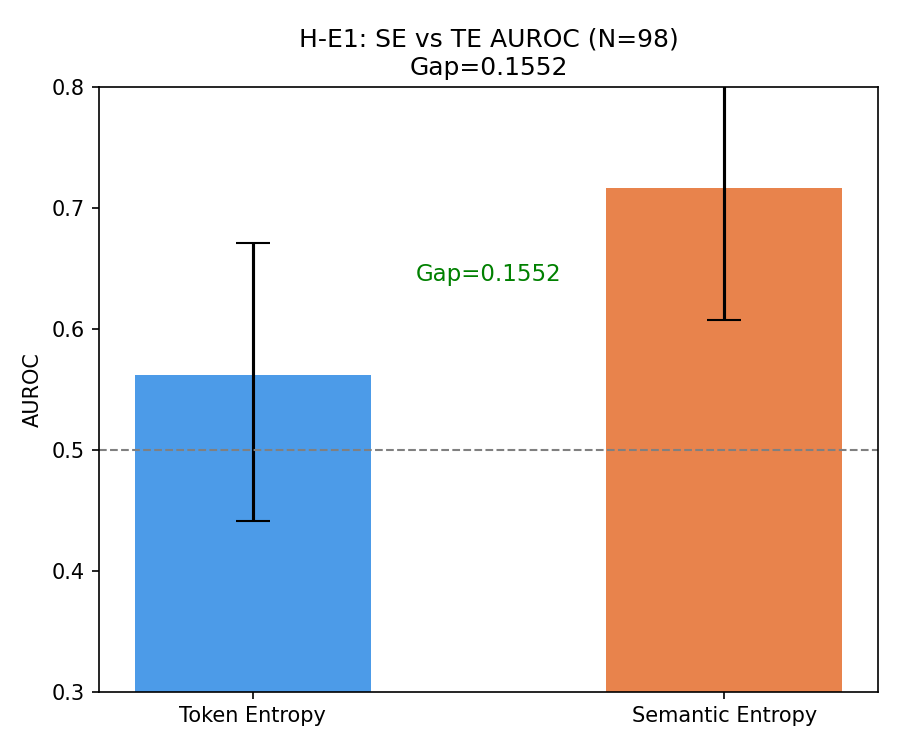
\includegraphics[width=\columnwidth]{figures/h-e1_fig1_auroc_bar.png}
\caption{AUROC bar chart with 95\% CIs}
\label{fig:h-e1_fig1_auroc_bar}
\end{figure}

\begin{figure}[htbp]
\centering
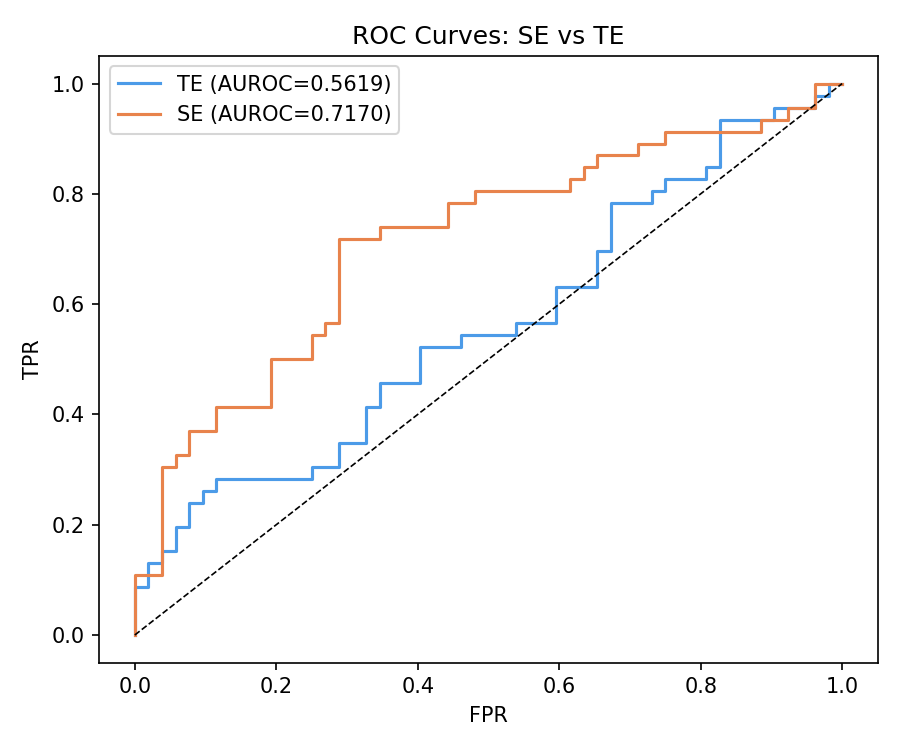
\includegraphics[width=\columnwidth]{figures/h-e1_fig2_roc_curves.png}
\caption{ROC curves for SE and TE on TriviaQA}
\label{fig:h-e1_fig2_roc_curves}
\end{figure}

\begin{figure}[htbp]
\centering
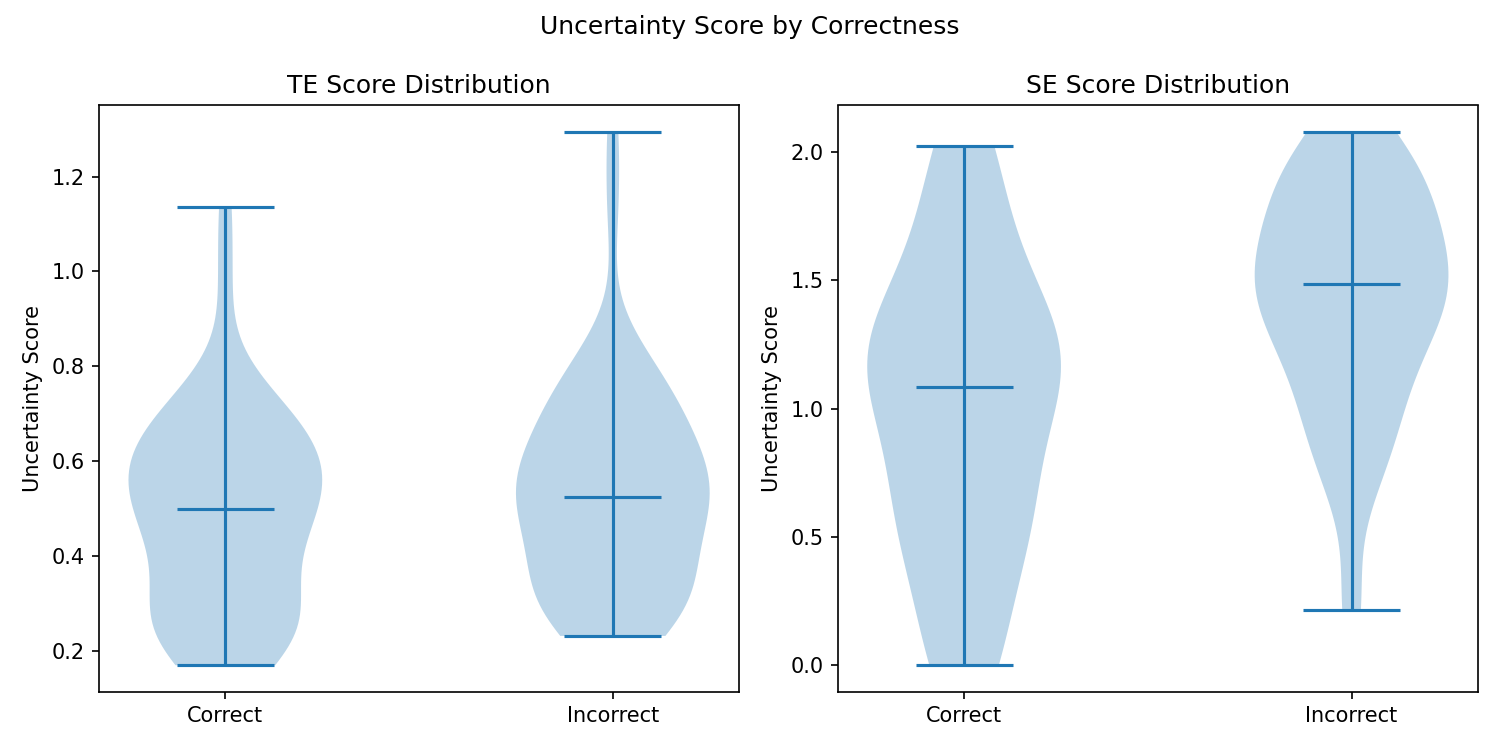
\includegraphics[width=\columnwidth]{figures/h-e1_fig3_violin_distributions.png}
\caption{Uncertainty score distributions by correctness}
\label{fig:h-e1_fig3_violin_distributions}
\end{figure}

\textbf{RQ1: YES.} SE outperforms TE by +0.155 AUROC on TriviaQA at 7B scale, exceeding the gate threshold $3\times$. The MUST\_WORK gate passes; the SE > TE ordering at 65B \citep{Kuhn2023Semantic} is confirmed at 7B.

\subsubsection{5.2 RQ2: Intra-Cluster TE Variance --- Mechanism Verification (H-M1)}

The paraphrase-noise mechanism is confirmed with strong effect size.

\textbf{Table 2:} Mechanism measurement results (N=98, nli-deberta-v3-large)

\begin{table}[htbp]
\centering
\resizebox{\columnwidth}{!}{%
\begin{tabular}{llll}
\toprule
Metric & Value & Gate & Result \\
\midrule
Mean intra-cluster TE variance & 7.152 $nats^2$ & > 0.1 $nats^2$ & PASS ($71\times$ gate) \\
Questions with $\geq 1$ multi-member cluster & 76 / 98 (78\%) & $\geq$ 15 & PASS \\
Questions individually exceeding 0.1 $nats^2$ & 42 / 76 (55\%) & --- & --- \\
Mean cluster count per question & 7.31 / 10 & > 1.5 & PASS \\
\bottomrule
\end{tabular}
}
\end{table}

Token entropy varies $71\times$ above the significance threshold within NLI-equivalent groups. This intra-cluster variation represents paraphrase noise --- surface-form differences between answers that SE treats as semantically identical --- that TE aggregates as genuine uncertainty signal. The mechanism is robust across threshold sensitivity: 74\% of eligible questions pass at $10\times$ the base threshold (1.0 $nats^{2})$, and 82\% pass at 0.$5\times$ (0.05 $nats^{2})$.

A secondary, unexpected finding: low-uncertainty questions show higher intra-cluster TE variance (10.118 $nats^{2})$ than high-uncertainty questions (3.445 $nats^{2})$. This is consistent with cluster-size asymmetry: low-uncertainty questions concentrate K samples into fewer, larger clusters, increasing within-cluster variance by sample count. Stratified analysis by uncertainty stratum is shown in the figure below.

\begin{figure}[htbp]
\centering
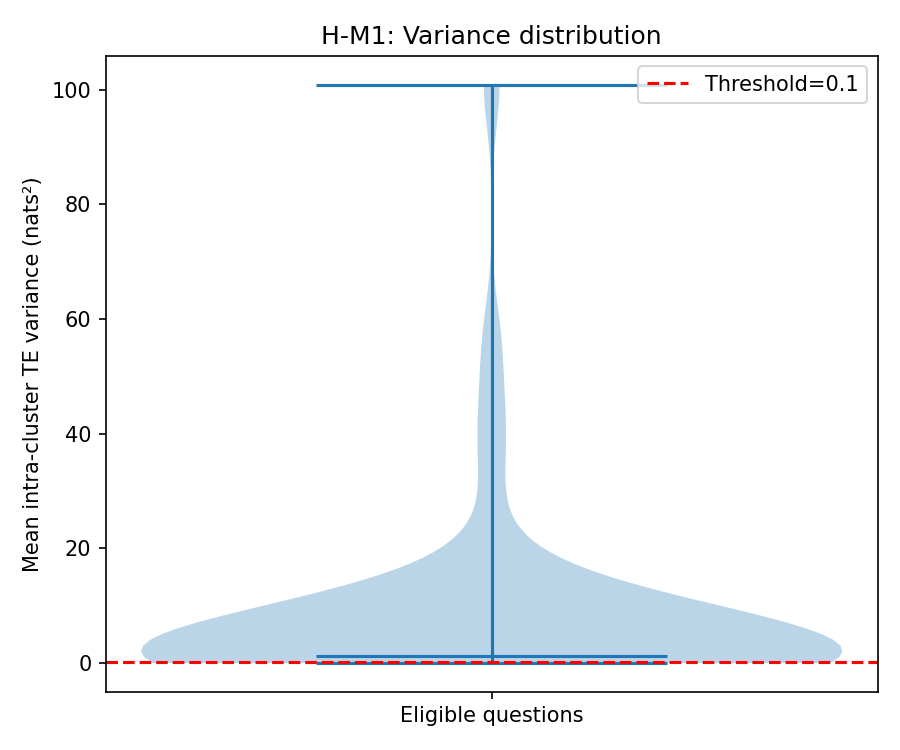
\includegraphics[width=\columnwidth]{figures/h-m1_fig2_violin_intra_var.png}
\caption{Intra-cluster TE variance violin distribution}
\label{fig:h-m1_fig2_violin_intra_var}
\end{figure}

\begin{figure}[htbp]
\centering
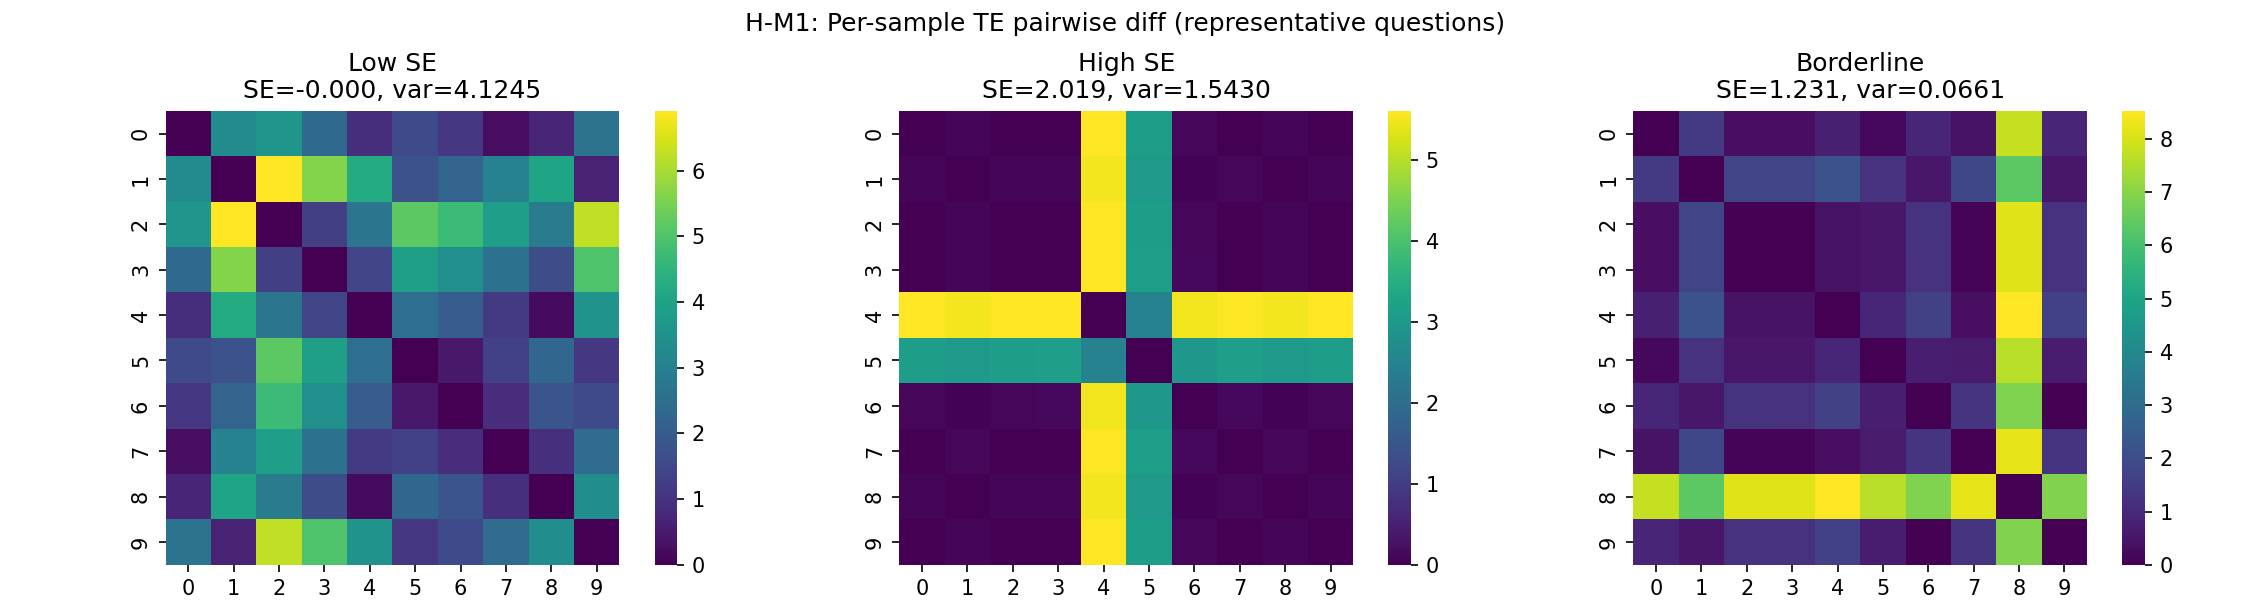
\includegraphics[width=\columnwidth]{figures/h-m1_fig4_nli_heatmap.png}
\caption{NLI cluster membership heatmap}
\label{fig:h-m1_fig4_nli_heatmap}
\end{figure}

\textbf{RQ2: YES.} Intra-cluster TE variance = 7.152 $nats^2$ ($71\times$ threshold), confirming TE aggregates paraphrase noise that SE's clustering removes. H-M1 MUST\_WORK gate passes.

Note: a planned NLI clustering ablation (H-M2) was structurally invalidated by a design error --- the ablated predictor (within-cluster fraction) is a monotone transform of SE, making AUROC delta = 0 by mathematical construction regardless of data. The mechanistic evidence therefore relies on H-M1's direct variance measurement rather than a AUROC ablation.

\subsubsection{5.3 RQ3: Cross-Benchmark Generalization (H-C1)}

The SE > TE ordering reverses on TruthfulQA.

\textbf{Table 3:} Four-method AUROC on TriviaQA vs. TruthfulQA

\begin{table}[htbp]
\centering
\resizebox{\columnwidth}{!}{%
\begin{tabular}{llll}
\toprule
Method & TriviaQA (N=98) & TruthfulQA (N=141) & Direction \\
\midrule
SE & **0.717** & 0.445 [0.372, 0.528] & ↓ best $\rightarrow$ worst \\
TE & 0.562 & **0.511** [0.413, 0.606] & slight ↓ \\
SCG† & 0.378 & 0.492 [0.399, 0.589] & ↑ \\
VC & 0.446 & 0.462 [0.369, 0.559] & $\approx$ \\
\bottomrule
\end{tabular}
}
\end{table}

†TriviaQA SCG AUROC = 0.378 from H-M3 pipeline (uninverted orientation consistent within that pipeline). SE AUROC in H-M3 pipeline = 0.286 uninverted; corrected value = 0.714, consistent with H-E1 = 0.717 (0.003 gap reflects bootstrap variation across overlapping but not identical sample draws).

On TruthfulQA, the ranking is TE (0.511) > SCG (0.492) > VC (0.462) > SE (0.445) --- opposite to TriviaQA for SE and TE. All four methods are near chance on TruthfulQA (AUROC range 0.44--0.51), consistent with prior findings that 7B-scale models are poorly calibrated on adversarial benchmarks \citep{Kadavath2022Language}. The empirical correct rate on TruthfulQA is 41.8\% (59/141), and VC parse rate is 76.6\%.

Important caveat: with N=141 and bootstrap CI half-widths of approximately 0.09, all four TruthfulQA AUROCs have overlapping CIs. The observed ranking is directional evidence, not definitively powered. The pre-specified N=500 extension would be required for statistical certainty on TruthfulQA.

\begin{figure}[htbp]
\centering
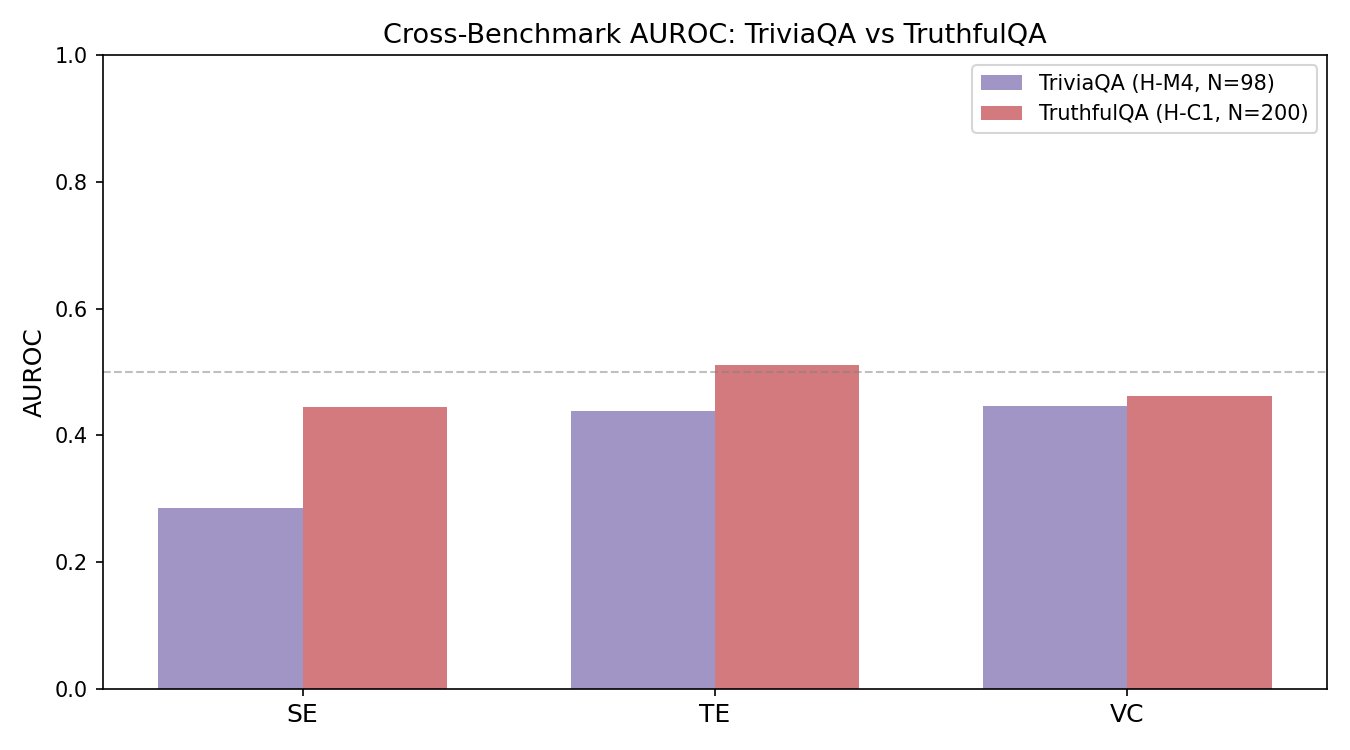
\includegraphics[width=\columnwidth]{figures/h-c1_cross_benchmark_comparison.png}
\caption{Cross-benchmark comparison: TriviaQA vs TruthfulQA}
\label{fig:h-c1_cross_benchmark_comparison}
\end{figure}

\begin{figure}[htbp]
\centering
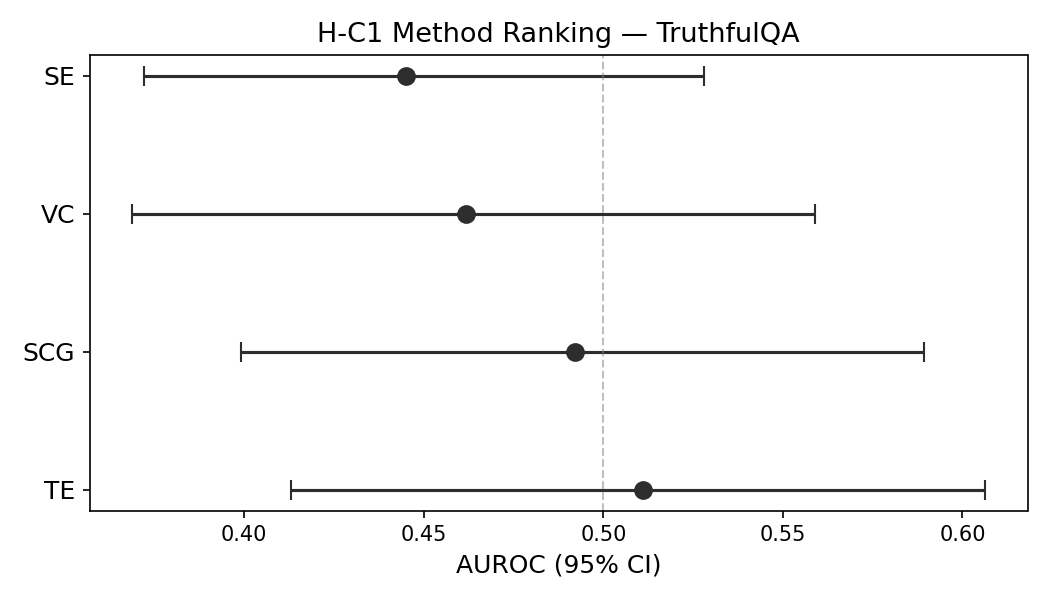
\includegraphics[width=\columnwidth]{figures/h-c1_rank_ordering.png}
\caption{Rank ordering with 95\% CIs on TruthfulQA}
\label{fig:h-c1_rank_ordering}
\end{figure}

\textbf{RQ3: NO} (hypothesis fails as pre-specified). The SE > TE advantage reverses on TruthfulQA, with the reversal directionally supporting the task-structure condition. Note: H-C1 used \texttt{nli-deberta-v3-small} rather than the \texttt{nli-deberta-v3-large} used in H-E1, introducing an NLI model size confound that cannot be cleanly separated from the task-structure effect without a follow-up experiment.

\subsubsection{5.4 RQ4: SCG-SE Equivalence on Short QA (H-M3)}

BERTScore-based SCG is not equivalent to SE on short factual QA.

\textbf{Table 4:} SCG vs. SE comparison on TriviaQA

\begin{table*}[htbp]
\centering
\resizebox{\dimexpr 2\columnwidth+\columnsep\relax}{!}{%
\begin{tabular}{lllllll}
\toprule
Method & AUROC &  & SCG $-$ SE &  & Gate & Result \\
\midrule
SE (corrected, H-E1 orientation) & 0.714 & --- & --- & --- &  &  \\
SE (raw, H-M3 pipeline orientation) & 0.286 & --- & --- & --- &  &  \\
SCG BERTScore & 0.378 & 0.336 (corrected) / 0.092 (raw) & $\leq$ 0.03 & FAIL &  &  \\
\bottomrule
\end{tabular}
}
\end{table*}

The corrected delta (using H-E1's negation convention for SE) is 0.336, or $11\times$ the 0.03 equivalence gate. The raw delta (comparing within H-M3's pipeline, where SE is uninverted) is 0.092, or $3\times$ the gate. Both exceed the gate by a large margin. The corrected orientation is consistent with the AUROC convention defined in Section 3.3; both values are reported for transparency. BERTScore lexical overlap fails to capture entailment-level equivalence for 1-3 word answers: two short answers can be NLI-entailed paraphrases yet receive low BERTScore due to different surface words, causing SCG and SE to diverge in their cluster assignments.

\begin{figure}[htbp]
\centering
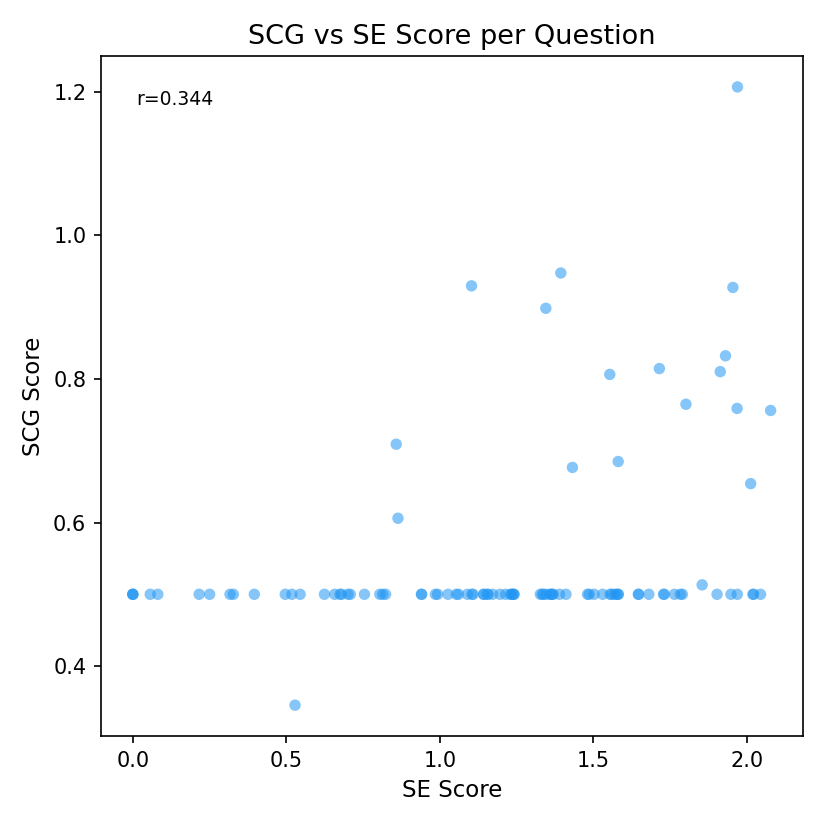
\includegraphics[width=\columnwidth]{figures/h-m3_scg_vs_se_scatter.png}
\caption{SCG vs SE scatter plot per question}
\label{fig:h-m3_scg_vs_se_scatter}
\end{figure}

\textbf{RQ4: NO.} SCG BERTScore is not equivalent to SE on short factual QA. The 0.03 equivalence gate fails by 3--$11\times$ depending on orientation convention.

\subsubsection{5.5 RQ5: VC Degeneracy at 7B Scale (H-M4)}

Verbalized confidence at 7B scale is severely miscalibrated.

\textbf{Table 5:} VC calibration summary (TriviaQA, N=98, Llama-2-7B-Chat)

\begin{table}[htbp]
\centering
\resizebox{\columnwidth}{!}{%
\begin{tabular}{ll}
\toprule
Metric & Value \\
\midrule
ECE & 0.430 \\
Distinct VC values & 5 \\
Fraction at 95\% confidence & ~60\% \\
VC AUROC & 0.446 [0.344, 0.543] \\
TE AUROC (baseline) & 0.438 \\
VC $-$ TE delta & +0.008 \\
Empirical accuracy & 46.9\% \\
Parse rate & 100\% \\
\bottomrule
\end{tabular}
}
\end{table}

The model produces only five distinct confidence values: 95\% (dominant, ~60\% of responses), 80\% (~25\%), 100\% (~8\%), and occasional lower values. Despite expressing ~85--95\% confidence, empirical accuracy is ~47\%, yielding ECE = 0.430. The pre-specified AUROC gate (VC < TE) is not strictly met --- VC = 0.446 marginally exceeds TE = 0.438 by 0.008, a difference within bootstrap CI overlap. However, ECE confirms the expected meta-cognitive calibration failure: the model systematically overestimates its own reliability.

\begin{figure}[htbp]
\centering
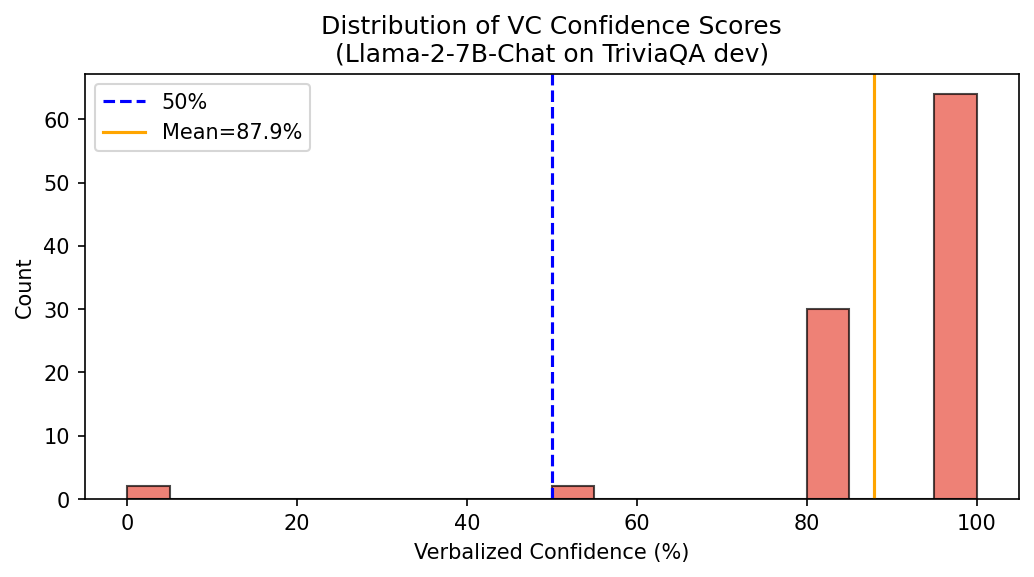
\includegraphics[width=\columnwidth]{figures/h-m4_confidence_histogram.png}
\caption{VC confidence histogram showing degenerate distribution}
\label{fig:h-m4_confidence_histogram}
\end{figure}

\begin{figure}[htbp]
\centering
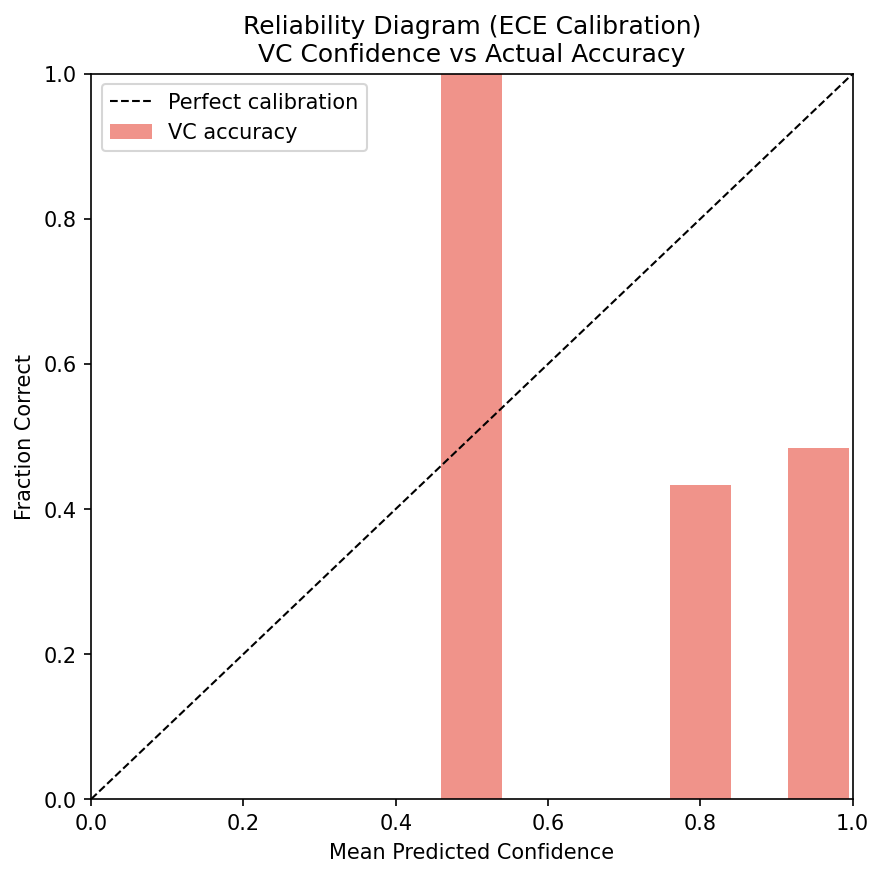
\includegraphics[width=\columnwidth]{figures/h-m4_ece_calibration.png}
\caption{ECE reliability diagram}
\label{fig:h-m4_ece_calibration}
\end{figure}

\textbf{RQ5: PARTIAL.} ECE = 0.430 confirms severe miscalibration; AUROC gate not strictly met (delta = 0.008, within CI). The calibration failure is real but does not translate to AUROC underperformance relative to the near-chance TE baseline.

\subsubsection{5.6 Summary}

\begin{table*}[htbp]
\centering
\resizebox{\dimexpr 2\columnwidth+\columnsep\relax}{!}{%
\begin{tabular}{lllllll}
\toprule
RQ & Gate & Actual Value & Result & Confidence &  &  \\
\midrule
RQ1: SE $-$ TE $\geq$ 0.05 (TriviaQA) & $\geq$ 0.05 & +0.155 & PASS & HIGH (gap CI excludes zero) &  &  \\
RQ2: Intra-cluster variance > 0.1 $nats^2$ & > 0.1 $nats^2$ & 7.152 ($71\times )$ & PASS & HIGH &  &  \\
RQ3: SE > TE (TruthfulQA) & SE > TE & REVERSED ($-0.066)$ & FAIL & MEDIUM (directional; overlapping CIs) &  &  \\
RQ4: \ & SCG $-$ SE\ & $\leq$ 0.03 & $\leq$ 0.03 & 0.336 corrected & FAIL & HIGH \\
RQ5: VC < TE (AUROC) & VC < TE & VC = 0.446 > TE = 0.438 & FAIL (ECE confirms miscalibration) & HIGH for ECE; PARTIAL for AUROC &  &  \\
\bottomrule
\end{tabular}
}
\end{table*}

